\PassOptionsToPackage{unicode=true}{hyperref} % options for packages loaded elsewhere
\PassOptionsToPackage{hyphens}{url}
%
\documentclass[english,jou]{apa6}
\usepackage{lmodern}
\usepackage{amssymb,amsmath}
\usepackage{ifxetex,ifluatex}
\usepackage{fixltx2e} % provides \textsubscript
\ifnum 0\ifxetex 1\fi\ifluatex 1\fi=0 % if pdftex
  \usepackage[T1]{fontenc}
  \usepackage[utf8]{inputenc}
  \usepackage{textcomp} % provides euro and other symbols
\else % if luatex or xelatex
  \usepackage{unicode-math}
  \defaultfontfeatures{Ligatures=TeX,Scale=MatchLowercase}
\fi
% use upquote if available, for straight quotes in verbatim environments
\IfFileExists{upquote.sty}{\usepackage{upquote}}{}
% use microtype if available
\IfFileExists{microtype.sty}{%
\usepackage[]{microtype}
\UseMicrotypeSet[protrusion]{basicmath} % disable protrusion for tt fonts
}{}
\usepackage{hyperref}
\hypersetup{
            pdftitle={Fractals are Cool},
            pdfauthor={Ben Chaloupka1, Tesufuai Sameshima1, \& Scott Wallner1},
            pdfkeywords={fractals, dwell time, growth sequence, decay sequence},
            pdfborder={0 0 0},
            breaklinks=true}
\urlstyle{same}  % don't use monospace font for urls
\usepackage{graphicx,grffile}
\makeatletter
\def\maxwidth{\ifdim\Gin@nat@width>\linewidth\linewidth\else\Gin@nat@width\fi}
\def\maxheight{\ifdim\Gin@nat@height>\textheight\textheight\else\Gin@nat@height\fi}
\makeatother
% Scale images if necessary, so that they will not overflow the page
% margins by default, and it is still possible to overwrite the defaults
% using explicit options in \includegraphics[width, height, ...]{}
\setkeys{Gin}{width=\maxwidth,height=\maxheight,keepaspectratio}
\setlength{\emergencystretch}{3em}  % prevent overfull lines
\providecommand{\tightlist}{%
  \setlength{\itemsep}{0pt}\setlength{\parskip}{0pt}}
\setcounter{secnumdepth}{0}

% set default figure placement to htbp
\makeatletter
\def\fps@figure{htbp}
\makeatother

% Manuscript styling
\usepackage{upgreek}
\captionsetup{font=singlespacing,justification=justified}

% Table formatting
\usepackage{longtable}
\usepackage{lscape}
% \usepackage[counterclockwise]{rotating}   % Landscape page setup for large tables
\usepackage{multirow}		% Table styling
\usepackage{tabularx}		% Control Column width
\usepackage[flushleft]{threeparttable}	% Allows for three part tables with a specified notes section
\usepackage{threeparttablex}            % Lets threeparttable work with longtable

% Create new environments so endfloat can handle them
% \newenvironment{ltable}
%   {\begin{landscape}\begin{center}\begin{threeparttable}}
%   {\end{threeparttable}\end{center}\end{landscape}}
\newenvironment{lltable}{\begin{landscape}\begin{center}\begin{ThreePartTable}}{\end{ThreePartTable}\end{center}\end{landscape}}

% Enables adjusting longtable caption width to table width
% Solution found at http://golatex.de/longtable-mit-caption-so-breit-wie-die-tabelle-t15767.html
\makeatletter
\newcommand\LastLTentrywidth{1em}
\newlength\longtablewidth
\setlength{\longtablewidth}{1in}
\newcommand{\getlongtablewidth}{\begingroup \ifcsname LT@\roman{LT@tables}\endcsname \global\longtablewidth=0pt \renewcommand{\LT@entry}[2]{\global\advance\longtablewidth by ##2\relax\gdef\LastLTentrywidth{##2}}\@nameuse{LT@\roman{LT@tables}} \fi \endgroup}

% \setlength{\parindent}{0.5in}
% \setlength{\parskip}{0pt plus 0pt minus 0pt}

% \usepackage{etoolbox}
\makeatletter
\patchcmd{\HyOrg@maketitle}
  {\section{\normalfont\normalsize\abstractname}}
  {\section*{\normalfont\normalsize\abstractname}}
  {}{\typeout{Failed to patch abstract.}}
\patchcmd{\HyOrg@maketitle}
  {\section{\protect\normalfont{\@title}}}
  {\section*{\protect\normalfont{\@title}}}
  {}{\typeout{Failed to patch title.}}
\makeatother
\shorttitle{Everything is Fractal}
\keywords{fractals, dwell time, growth sequence, decay sequence}
\usepackage{dblfloatfix}


\usepackage{csquotes}
\ifnum 0\ifxetex 1\fi\ifluatex 1\fi=0 % if pdftex
  \usepackage[shorthands=off,main=english]{babel}
\else
  % load polyglossia as late as possible as it *could* call bidi if RTL lang (e.g. Hebrew or Arabic)
  \usepackage{polyglossia}
  \setmainlanguage[]{english}
\fi

\title{Fractals are Cool}
\author{Ben Chaloupka\textsuperscript{1}, Tesufuai Sameshima\textsuperscript{1}, \& Scott Wallner\textsuperscript{1}}
\date{}


\affiliation{\vspace{0.5cm}\textsuperscript{1} University of Oregon}

\abstract{
Fractals can be described as geometric objects which contain self similarity and scale invariance. Fractal objects and fractal properties are pervasive in nature. Many processes which involve replication or growth can be modeled with fractal mathematics. The formalized mathematics of fractals has been used as an analog for complexity, an important property related to human cognition. Studies have shown that human perception has evolved to process fractals fluently, as well as exhibit aesthetic preferences for fractals. The experience of fractals in a number of domains have proven to be therapeutically useful. Previous studies have used independent and static fractal images to investigate the relationship between, fractals, complexity and human perception. This study employs a Dwell Time Paradigm to present self paced slide shows of dynamic fractals in an unfolding process of iterative growth and decay. Results of measured looking or dwell times show that participants prefer viewing fractals as they grow through phases of increasing complexity compared to decay phases of decreasing complexity. Longer dwell times for higher complexity may indicate that human perception is captured by the surprising or novel nature of a fractal's iterative growth process. This study is the first to use a novel presentation of dynamic fractal processes to explore fractal fluency and aesthetic preference. Results from 16 participants prove that dynamic fractals can be integrated into the well established dwell time paradigm. These findings can be used to develop new techniques for utilizing fractals as therapeutic tools.
}



\begin{document}
\maketitle

\hypertarget{introduction}{%
\section{Introduction}\label{introduction}}

Fractal is a term originally derived to describe the \enquote{roughness,} (Mandelbrot, 1989) of objects, surfaces, or textures. Fractal properties are pervasive throughout nature (Losa, 2009) and can be identified in the texture of clouds and mountains, in the branching pattern of trees and lightning, in the meandering shape of rivers and blood vessels. These fractal properties are identified by their self-similarity and scale invariance. Self-similarity implies that a part of the structure maintains the same structure or pattern as the whole. For example, if one were to zoom in on a small stretch of coastline, the jagged edges would look similar to the jaggedness of the coastline from a broader view. Likewise, a small section of a fern is nearly identical to the branching shape of the entire fern.

\begin{figure}

{\centering 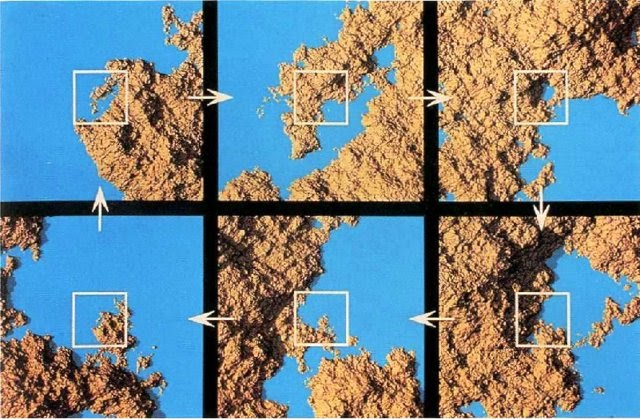
\includegraphics[width=0.3\linewidth]{/Users/bchaloup/Documents/Fall 2020/EDLD651/final_project/paper/paper_images/coast} 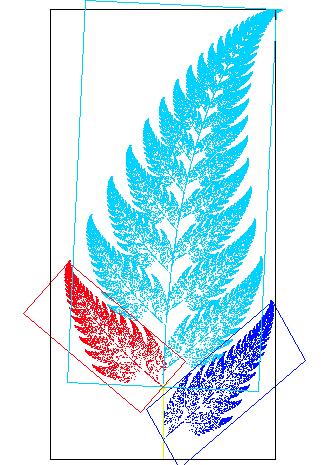
\includegraphics[width=0.3\linewidth]{/Users/bchaloup/Documents/Fall 2020/EDLD651/final_project/paper/paper_images/fractalfern} 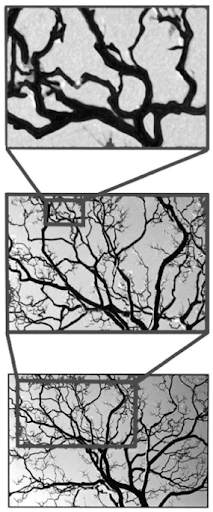
\includegraphics[width=0.3\linewidth]{/Users/bchaloup/Documents/Fall 2020/EDLD651/final_project/paper/paper_images/spooky} 

}

\caption{ }\label{fig:unnamed-chunk-1}
\end{figure}

Scale-invariance is a related mathematical property which can be applied to objects that do not change across different scales; there is a similar patterm at all levels of magnification. Expressed more intuitively, scale invariance implies that it does not matter at which scale one views and object or observes a process, because the object or process contains a commonality at all scales.

It is interesting and important to note that the concept of fractal properties can be applied to objects like a snowflake, but also processes, like the crystallization of the snowflake. Crystals are created by repeating a simple process over and over in a feedback loop. A crystal starts with a tiny bit of structure, and that structure is repeated, growing on itself using the same pattern or rule for growth. This can be seen quite obviously in objects that are themselves fractals, such as the branching process of trees, but other natural processes follow the rules of fractals. Hurricanes, avalanches, the diffusion of molecules in solution, the dissolving of porous rock, the electrical breakdown of dialectics, and in the growth of our lungs and brains. Strikingly fractal properties can be found in statistical systems or distributions of word usage, foraging behaviors, rock size and in the frequency of scientific journal citations, and network outages of the internet. (Wiki, scale invariance) The underlying principle of fractals is that a simple process can through infinitely many iterations to become a very complex process. Many processes which involve bifurcation, splitting, replication and growth can be fractal mathematics and geometry. Fractal mathematics can model these complex systems by searching for the simple rules or laws that drive these processes. (\url{http://pages.cs.wisc.edu/~ergreen/honors_thesis/fractal.html})

In addition to inventing the term fractal, Mandelbrot developed a mathematics and geometry of fractals. He devised a way to model and generate complex systems with a simple mathematical rule that could be run repeatedly or iterated on itself. These iterative processes essentially use a rule to take an initial condition or state, change or modulate it, then put the resulting updated state back into the rule to generate another new state. This can be repeated infinitely and often results in high complex objects or systems. Fractal mathematics have continued to be developed and utilized in mathematics, physics, biology, chemistry, and engineering.A recent application of fractal mathematics is utilized in computer generated images and models. By starting with a simple algorithm, a mathematical equation or rule, graphic artists and programmers can create highly complex models of natural systems.

By replicating the fractal processes in nature, computer programs can generate digital forests, mountain ranges, and coastlines. These images can be found in movies and video games. Similarly scientists and engineers can use fractal mathematics to generate models of complex systems that accurately represent patterns and processes in weather, cosmology, electronics, and statistics.

Two premiere examples of these mathematical or statistical fractals can be seen in the Koch Curve and the Cantor Set. In each case an image is created by starting with a single line segment and a rule for changing that line segment. The cantor set can be visualized by displaying each cycle of the process of iteration together. First a single line segment is displayed. The Cantor Set rule divides the segment in three equal sections and removes the middle section, leaving two line segments each one third of the original length and separated by a space equal to one third of the original line segment. The two separated line segments of the 2nd order iteration can be displayed beneath the original first order line segment. The rule, dividing and removing a portion of the line segment is applied to the two new line segments. Each of these line segments is divided into thirds and the middle third is removed. This results in four new smaller line segments spaced in a proportion equal to the previous two line segments. These four line segments are again displayed under the two line segments. This process can be repeated infinitely many times, dividing and removing segments at each iteration. When displayed together, we are able to visualize the repeating pattern which relates to the simple unchanging rule. This is an intuitive way to represent the properties of self-similarity, scale invariance, and iterative growth rules of fractals. A similar example is the Koch Curve. Again we start with a single line segment, but define a new rule to change that line segment through each iteration. Like the Cantor set, the line segment is divided into thirds, but instead of just removing the middle third which results in two new line segments, we bridge the middle third with two line segments that compose two sides of an isosceles triangle which spans the removed middle third of the original line. This new segmented line of the 2nd order iteration appears as a line with a triangular bump or protrusion in the middle. The entire segment is composed of four connected line segments. Again, by using the same algorithmic rule, divide a segment into thirds and span the removed middle third with an isosceles angle, and is applied to all four of the line segments created by the first iterative change. Now each of these four line segments will include an angular bump or peak that spans their middle third.These results in a set of 16 angular connected line segments. Just as we did with the cantor set, and can do with all fractal growth iterations, we can continue applying the rule to the updated condition of the object. This time, unlike the cantor set which displays all the iterations together, a single, new object is produced at each iteration. We can visualize the growth process by displaying a few of these objects together.

\begin{figure}

{\centering 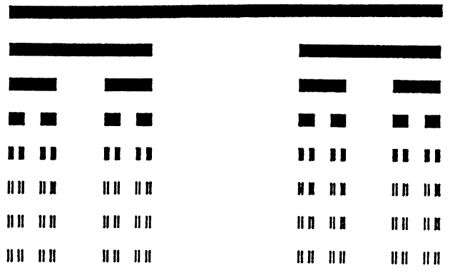
\includegraphics[width=0.5\linewidth]{/Users/bchaloup/Documents/Fall 2020/EDLD651/final_project/paper/paper_images/bars} 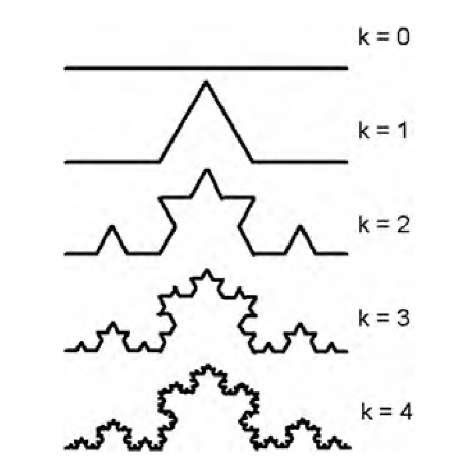
\includegraphics[width=0.5\linewidth]{/Users/bchaloup/Documents/Fall 2020/EDLD651/final_project/paper/paper_images/star} 

}

\caption{ }\label{fig:unnamed-chunk-2}
\end{figure}

There are numerous examples of these types of geometric transformations which result in beautiful and striking constructions. Some well known fractal geometries are known as, The Dragon Curve, Sierpinski Triangle, and Hilbert Curve. These examples show the diversity of implementations of fractal properties in geometry. The variety of initial conditions and algorithmic rules result in an astounding array of complex objects which have real world applications and instantiations.

\begin{figure}

{\centering 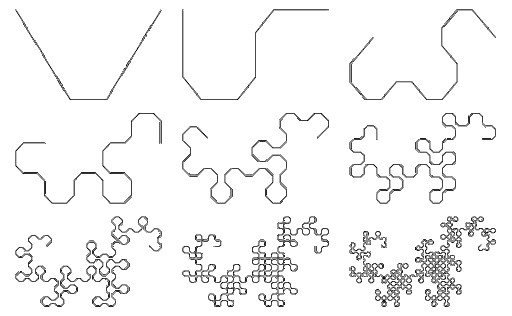
\includegraphics[width=0.3\linewidth]{/Users/bchaloup/Documents/Fall 2020/EDLD651/final_project/paper/paper_images/squigly} 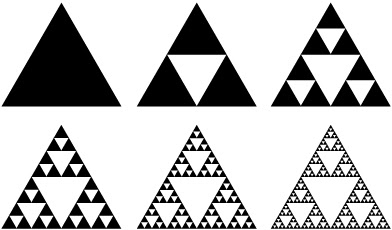
\includegraphics[width=0.3\linewidth]{/Users/bchaloup/Documents/Fall 2020/EDLD651/final_project/paper/paper_images/triangle} 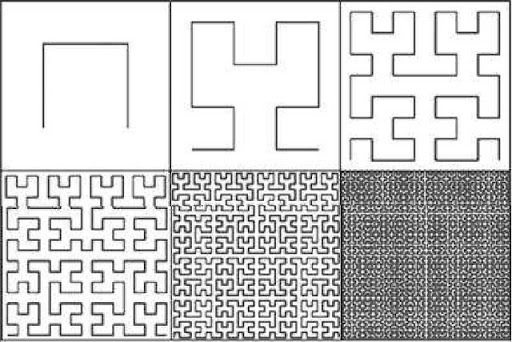
\includegraphics[width=0.3\linewidth]{/Users/bchaloup/Documents/Fall 2020/EDLD651/final_project/paper/paper_images/maze} 

}

\caption{ }\label{fig:unnamed-chunk-3}
\end{figure}

These examples provide intuition about fractal processes and properties for anyone who may not have any experience or deep knowledge of the underlying mathematics. Even a surface level experience of the properties of fractals allow one to engage with challenging and complex mathematical ideas. One such idea critical to fractal mathematics is dimensionality. Many learn and understand the concept of dimension as it is traditionally explained in mathematics. Most will understand that a line is considered as one dimensional and a plane as two dimensional. One dimension, as in the line, allows for movement or positions in one degree of freedom, left and right or forward and backward. Two dimensions allow for two degrees of freedom, left-right and forward-backward, or as we often see in the plane of a map, North, South, East, West. It is also intuitive to relate to three dimensions, which describe objects and space which contains the two dimensions of a plane, but also a third degree of freedom as up and down. Fractal mathematics introduces a concept of dimensionality that can exist between these integer values of 1, 2, or 3 dimensions. A fractal like the Dragon Curve or Koch Curve can have a dimensionality between 1 and 2, such as 1.2, 1.5, or 1.74823. At first this concept feels counter intuitive. The non-integer dimensionality occurs because the length of the curve between any two points on the Koch snowflake is effectively infinite. No small piece of it is line-like, but rather it is composed of an infinite number of segments joined at different angles. The fractal dimension of a curve can be explained intuitively by thinking of a fractal line as an object too detailed to be one-dimensional, but too simple to be two-dimensional. (\url{https://en.wikipedia.org/wiki/Fractal_dimension}) Another way to understand this is to consider the process by which the Koch Curve is constructed. As we continually modulate the object through iterations, we can add an infinite number of additional line segments which create innumerable jagged peaks. The Koch Curve which began with a one dimensional line will continue to take up more and more space, eventually filling a two dimensional area.

\begin{figure}

{\centering 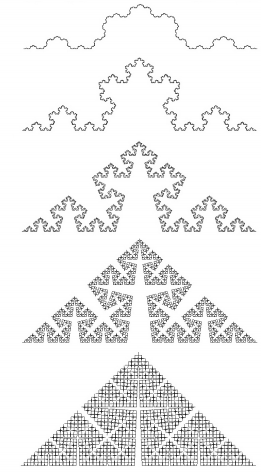
\includegraphics[width=0.9in,height=0.3\textheight]{/Users/bchaloup/Documents/Fall 2020/EDLD651/final_project/paper/paper_images/morefractals} 

}

\caption{ }\label{fig:unnamed-chunk-4-1}
\end{figure}
\begin{figure}

{\centering 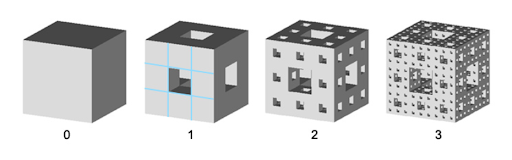
\includegraphics[width=1.71in,height=0.3\textheight]{/Users/bchaloup/Documents/Fall 2020/EDLD651/final_project/paper/paper_images/square} 

}

\caption{ }\label{fig:unnamed-chunk-4-2}
\end{figure}

In this way we can realize that the Koch Curve is neither one or two dimensional, it is somewhere in between. Using fractal mathematics invented by Mandelbrot, we can calculate the dimensionality of any fractal including the Koch and Dragon Curves which have dimensionalities of 1.262 and 1.5236 respectively. Similarly an object which begins as a two dimensional fractal, can be iterated to grow into the third dimension and have a calculated dimension between 2 and 3. Thus, dimensionality can be considered as the space filling capacity of a fractal. But seen another way, fractal dimension is a ratio providing a statistical index of complexity comparing how detail in a pattern changes with the scale at which it is measured. The connection between fractal dimension and complexity has been used to understand how biological systems including human perception contain or interact with complexity.

Calculating fractal dimension is not restricted to geometric or statistical fractals as described above. One can also calculate a D value, fractal dimension of natural objects like coastlines, the outlines of clouds, or the silhouettes of mountain ranges on the horizon. These ideas have been rigorously developed and investigated, exemplified in the University of Oregon's Dr.~Richard Taylor theory of Fractal Fluency. Simply put, human vision has not only adapted to efficiently process and perceive the dimensionality of fractals in nature, but has evolved to prefer fractals of a certain dimensional range.

To date there have been numerous research studies which explore the aesthetic preferences for fractals of different dimensions. Studies have included methods which present participants with a two alternative forced choice task of two fractals of differing dimension. Participants select the fractal image they prefer aesthetically and after viewing many pairs with differing dimensions, statistics are used to calculate the most preferred dimensionality range across participants. The overarching results of previous research have shown that humans, both adults and children prefer fractals within a range of dimensions that coincide with the fractal dimension that is found in natural objects and scenes, usually between 1.3 and 1.5.Remembering that fractal dimension is an analog for complexity, we can conclude that most humans prefer a moderate level of complexity compared to low or high complexity near the extremes. A secondary analysis of fractal fluency has shown that humans often also prefer fractal images to non-fractal images and that we prefer fractals which more closely resemble natural images to fractals which are geometrically exact. (Spehar, Clifford, Newell, \& Taylor, 2003) Extensions on these research findings have led to the use of fractal images in therapeutic applications. Studies have shown some benefits of experiencing fractals, including physiological responses in EEG measurement of brain activity while viewing fractals (Hagerhall et al., 2015), the reduction of stress using fractal art and architecture (Taylor, 2006) and even in the experience of hearing fractal melodies (Beauvois, 2007). There appears to be a clear link between, the fractal's representation of complexity, the connection with natural objects and processes, and the human mind.

Despite many studies which explore the link between fractals, complexity, and human perception and aesthetics, there are continued adaptations and developments to the body of work. This study attempts to address a gap in the way these ideas are explored. Here we employ a novel presentation of fractal images which has yet to be tested or analyzed. Specifically most studies of fractal fluency and aesthetic preference have used static independent fractal images. This means, participants are usually restricted to the selection of a single fractal image in a given trial, and an unrelated or random image in the next trial.

\begin{figure}

{\centering 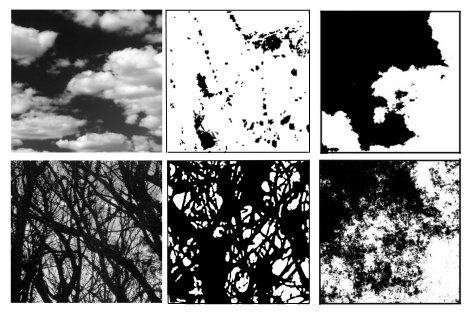
\includegraphics[width=0.3\linewidth]{/Users/bchaloup/Documents/Fall 2020/EDLD651/final_project/paper/paper_images/blotches} 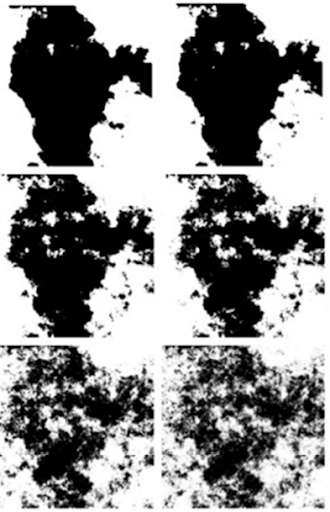
\includegraphics[width=0.3\linewidth]{/Users/bchaloup/Documents/Fall 2020/EDLD651/final_project/paper/paper_images/moreblotches} 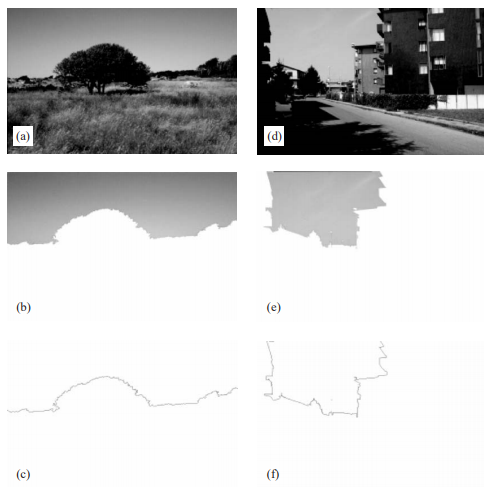
\includegraphics[width=0.3\linewidth]{/Users/bchaloup/Documents/Fall 2020/EDLD651/final_project/paper/paper_images/deconstruction} 

}

\caption{ }\label{fig:unnamed-chunk-5}
\end{figure}

However our natural experience of the world is not so static, fragmented and simple, it is often dynamic, cohesive and alive. To create a more lifelike experience of fractals we present participants with the unfolding process of a fractal as it is iterated through its process of changing in complexity. By allowing participants to view a series of fractal images which increase and decrease in complexity we can more effectively understand the human experience of fractals that more closely resemble the dynamic process of life. The results of this study may provide new and exciting understandings related to fractal fluency and preference as well as inspire the development of therapeutic applications of fractals.

\hypertarget{methods}{%
\section{Methods}\label{methods}}

Participants viewed self paced slideshows of fractal images in sequences of iterative growth and decay phases as well as a random ordering. The time spent viewing each image was measured as a Dwell Time, following the procedures of Baldwin et al.~2019. A set of images were generated for each of fourteen different fractal types iterated from 4 to 9 times. Each participant viewed a sequential slideshow and a random slideshow. Sequential slideshows presented each fractal type through phases of growth and decay from the least complex to most complex iterations and back down from most complex to least complex. Random slideshows presented the entire set of fractal images in random order. Six participants viewed Sequential Slideshow A, starting with Fractal Type 1 to Type 14, and Random Slideshow A starting with Fractal Image 1 to Image 174. The remaining 10 participants viewed Sequential Slideshow B, starting with Fractal Type 14 to Type 1, and Random Slideshow B starting with Fractal Image 174 to Image 1. This counterbalancing was included to address the findings of previous dwell time studies in which participants dwell times systematically decrease through the slideshow. In this way, the same fractal types were not always seen at the beginning or end of the slideshow. This balancing was then reversed in analysis so that each fractal type and the corresponding dwell times could be analyzed for the entire set of 16 participants together. Fractal images were generated using Wolfram Mathematica and slideshows were programmed using PsychoPy 3.

\begin{figure}

{\centering 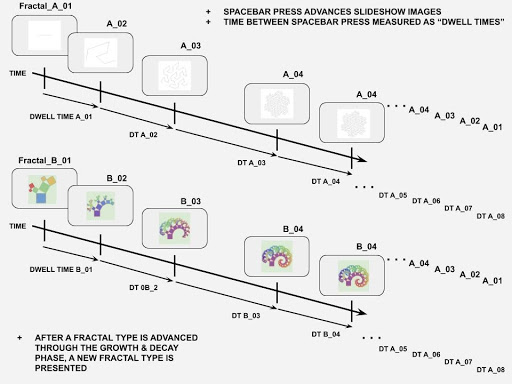
\includegraphics[width=1.71in,height=0.25\textheight]{/Users/bchaloup/Documents/Fall 2020/EDLD651/final_project/paper/paper_images/task_outline} 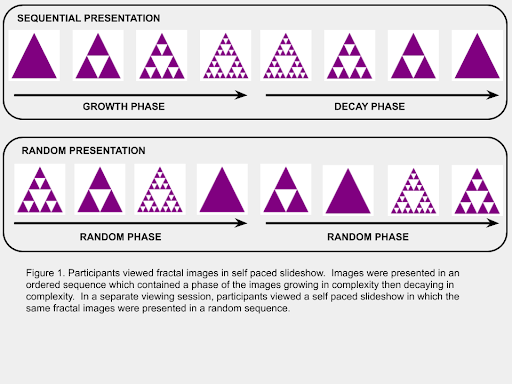
\includegraphics[width=1.71in,height=0.25\textheight]{/Users/bchaloup/Documents/Fall 2020/EDLD651/final_project/paper/paper_images/fractal_direction} 

}

\caption{ }\label{fig:unnamed-chunk-6}
\end{figure}

\hypertarget{participants}{%
\subsection{Participants}\label{participants}}

The study recruited 16 healthy young adults ages 16-35 through the UO SONA recruitment system. All participants had normal or corrected to normal vision with no history of neurological damage.

\hypertarget{data-analysis}{%
\subsection{Data analysis}\label{data-analysis}}

We used R (Version 3.6.3; R Core Team, 2019) and the R-packages \emph{\}here} {[}@\}R-here{]}, \emph{dplyr} (Version 1.0.2; Wickham et al., 2020), \emph{forcats} (Version 0.5.0; Wickham, 2020a), \emph{ggplot2} (Version 3.3.2; Wickham, 2016), \emph{janitor} (Version 2.0.1; Firke, 2020), \emph{knitr} (Version 1.30; Xie, 2015), \emph{papaja} (Version 0.1.0.9997; Aust \& Barth, 2020), \emph{purrr} (Version 0.3.4; Henry \& Wickham, 2020), \emph{readr} (Version 1.4.0; Wickham \& Hester, 2020), \emph{rio} (Version 0.5.16; Chan, Chan, Leeper, \& Becker, 2018), \emph{stringr} (Version 1.4.0; Wickham, 2019), \emph{tibble} (Version 3.0.4; Müller \& Wickham, 2020), \emph{tidyr} (Version 1.1.2; Wickham, 2020b), and \emph{tidyverse} (Version 1.3.0; Wickham, Averick, et al., 2019) for all our analyses.

\hypertarget{results}{%
\section{Results}\label{results}}

\begin{table*}[htbp]

\begin{center}
\begin{threeparttable}

\caption{\label{tab:tbyp}Descriptive statistics of dwell times by participant and direction}

\begin{tabular}{llll}
\toprule
Participant & Sequence Direction & Mean Dwell Time (s) & SD Dwell Time (s)\\
\midrule
a & Decay & 1.41 & 1.15\\
a & Growth & 3.44 & 1.91\\
a & Random & 1.48 & 1.08\\
b & Decay & 1.16 & 0.50\\
b & Growth & 1.56 & 0.96\\
b & Random & 0.75 & 0.33\\
c & Decay & 0.62 & 0.13\\
c & Growth & 0.70 & 0.23\\
c & Random & 0.78 & 0.26\\
d & Decay & 0.42 & 0.12\\
d & Growth & 0.45 & 0.18\\
d & Random & 0.52 & 0.15\\
e & Decay & 0.76 & 0.12\\
e & Growth & 0.78 & 0.12\\
e & Random & 0.82 & 0.11\\
f & Decay & 0.75 & 0.14\\
f & Growth & 0.79 & 0.14\\
f & Random & 0.75 & 0.12\\
g & Decay & 0.60 & 0.07\\
g & Growth & 0.61 & 0.08\\
g & Random & 0.73 & 0.18\\
h & Decay & 0.45 & 0.11\\
h & Growth & 0.47 & 0.12\\
h & Random & 0.62 & 0.14\\
i & Decay & 1.21 & 0.42\\
i & Growth & 1.23 & 0.31\\
i & Random & 1.12 & 0.34\\
j & Decay & 0.81 & 0.18\\
j & Growth & 0.88 & 0.20\\
j & Random & 1.33 & 0.33\\
k & Decay & 0.84 & 0.13\\
k & Growth & 0.92 & 0.19\\
k & Random & 1.27 & 0.52\\
l & Decay & 0.59 & 0.17\\
l & Growth & 0.74 & 0.23\\
l & Random & 0.73 & 0.23\\
m & Decay & 0.75 & 0.31\\
m & Growth & 1.01 & 0.32\\
m & Random & 0.65 & 0.15\\
n & Decay & 0.49 & 0.11\\
n & Growth & 0.57 & 0.15\\
n & Random & 0.72 & 0.17\\
o & Decay & 0.42 & 0.06\\
o & Growth & 0.43 & 0.07\\
o & Random & 0.41 & 0.04\\
p & Decay & 0.49 & 0.11\\
p & Growth & 0.57 & 0.15\\
p & Random & 1.01 & 0.19\\
\bottomrule
\addlinespace
\end{tabular}

\begin{tablenotes}[para]
\normalsize{\textit{Note.} Participant means and standard deviations for dwell times by sequence direction (growth, decay, or random). All units are in seconds (s).}
\end{tablenotes}

\end{threeparttable}
\end{center}

\end{table*}

Descriptive statistics for each participant by direction of sequence are shown in Table~\ref{tab:tbyp}.

\begin{figure}
\centering
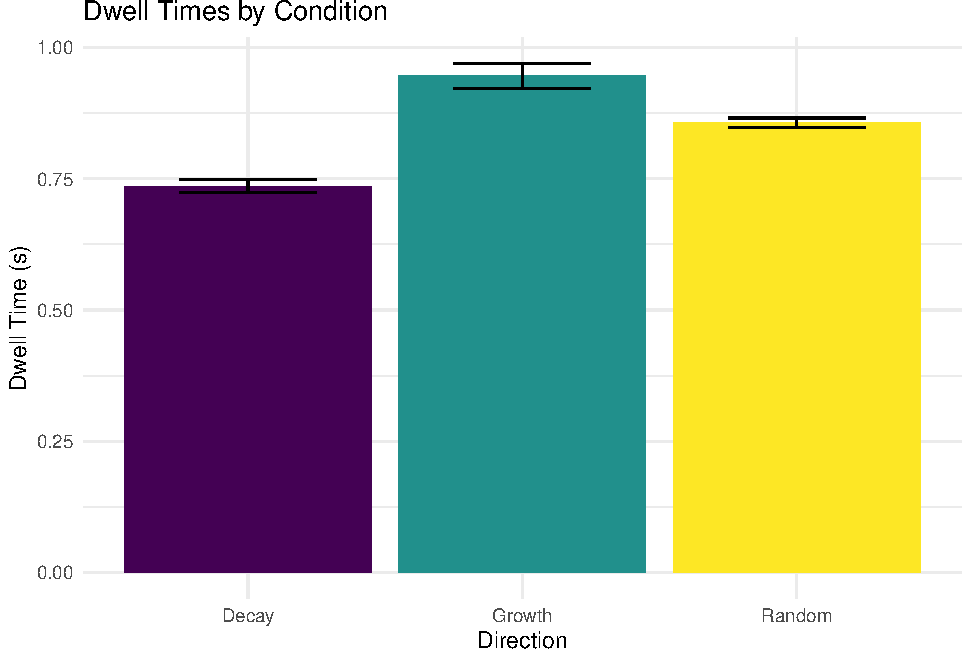
\includegraphics{paper_papaja_files/figure-latex/main-1.pdf}
\caption{\label{fig:main}Error bars represent standard errors.}
\end{figure}

A one-way ANOVA was conducted to examine the effect of fractal presentation directions on dwell times. There was a significant effect of direction on dwell time, \(F(2, 5,565) = 42.68\), \(\mathit{MSE} = 0.36\), \(p < .001\), \(\hat{\eta}^2_G = .015\). These results demonstrate that growth conditions showed significantly longer dwell times compared to the decay or random directional conditions. These results are depicted in Figure~\ref{fig:main}.

\begin{figure}
\centering
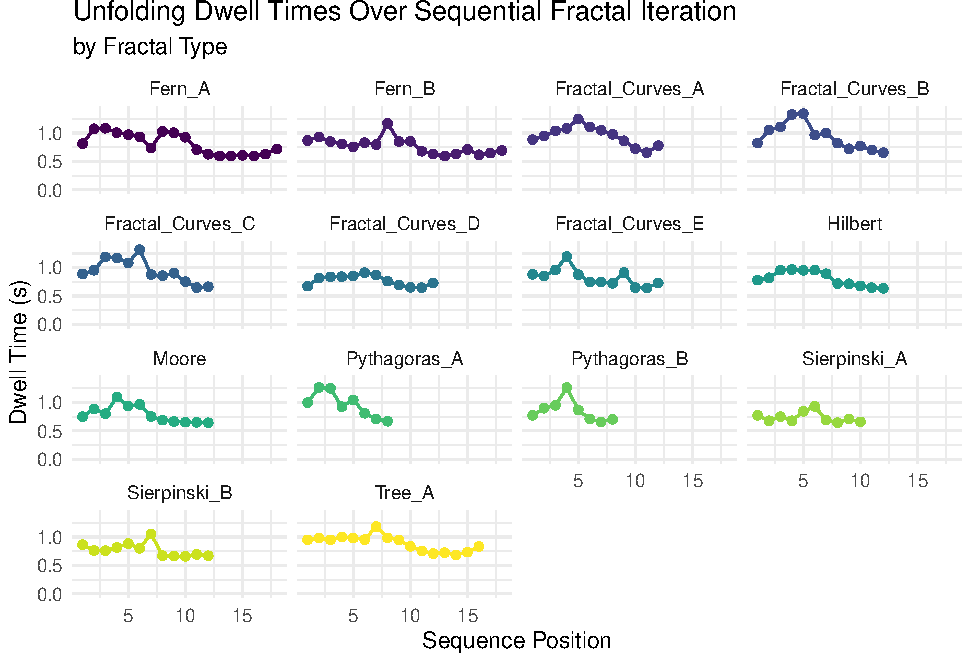
\includegraphics{paper_papaja_files/figure-latex/ftfig-1.pdf}
\caption{\label{fig:ftfig}Dwell times by fractal type and sequence position.}
\end{figure}

Additionally, we conducted a two-way ANOVA with sequence position and fractal type as the factors. There was a significant main effect of fractal type, \(F(13, 2,697) = 2.30\), \(\mathit{MSE} = 0.53\), \(p = .005\), \(\hat{\eta}^2_G = .011\), and a main effect of sequence position, \(F(8, 2,697) = 2.02\), \(\mathit{MSE} = 0.53\), \(p = .041\), \(\hat{\eta}^2_G = .006\). There was not a significant interaction, \(F(65, 2,697) = 0.37\), \(\mathit{MSE} = 0.53\), \(p > .999\), \(\hat{\eta}^2_G = .009\). These results suggest that different fractal types elicit different dwell times, and that dwell times vary significantly by position in the growth-decay sequence, but these effects are independent of one another. These results are represented in Figure~\ref{fig:ftfig}.

\begin{figure}
\centering
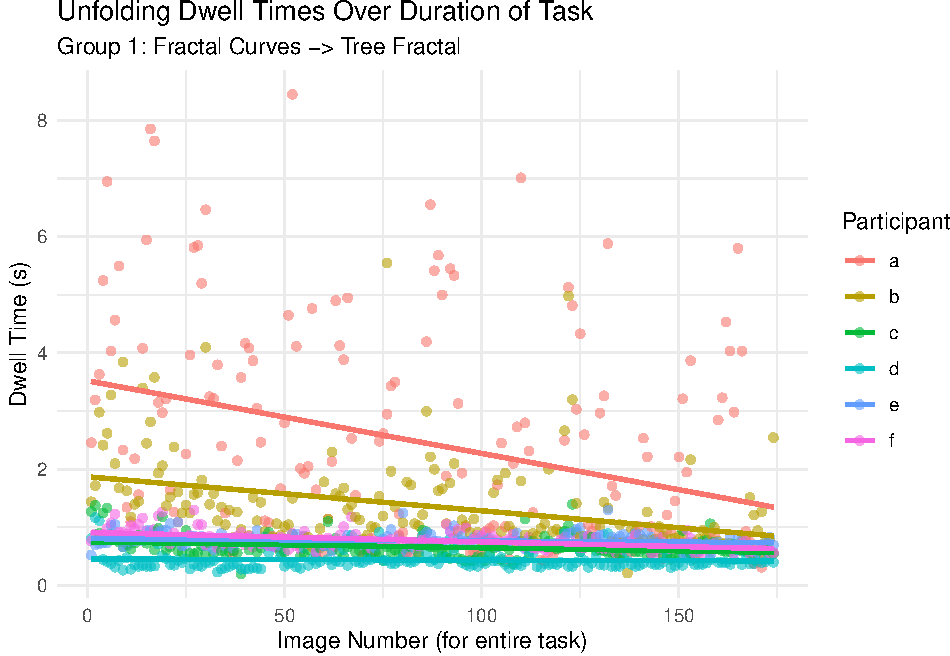
\includegraphics{paper_papaja_files/figure-latex/fatigue1-1.pdf}
\caption{\label{fig:fatigue1}Dwell times over length of entire session for group 1. This group saw the fractal curves first and the tree fractal last.}
\end{figure}

\begin{figure}
\centering
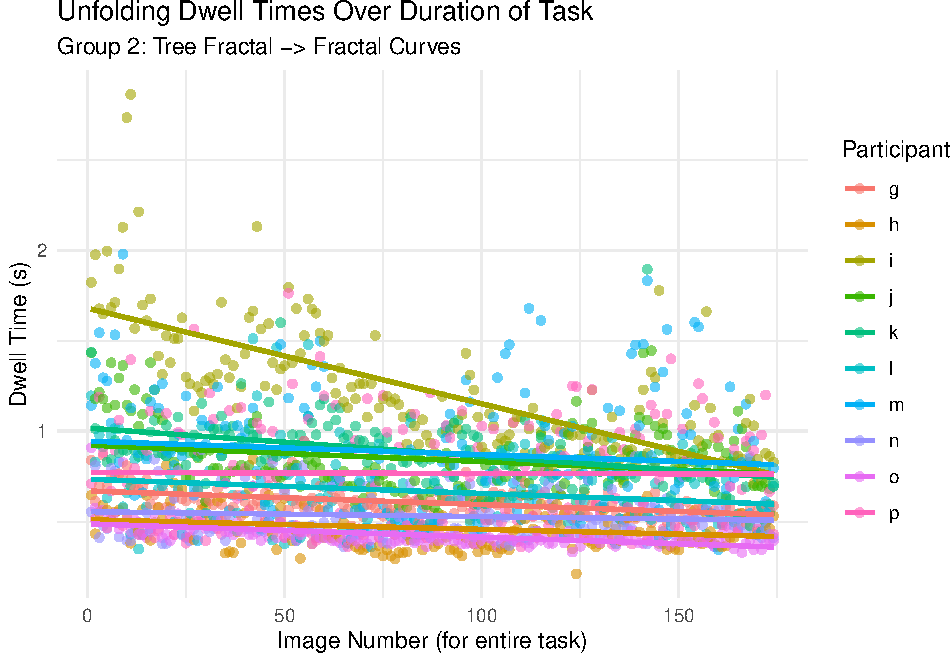
\includegraphics{paper_papaja_files/figure-latex/fatigue2-1.pdf}
\caption{\label{fig:fatigue2}Dwell times over length of entire session for group 2. This group saw the tree fractal first and the fractal curves last.}
\end{figure}

Figure~\ref{fig:fatigue1} plots the dwell times over the course of the study for participant group 1, and Figure~\ref{fig:fatigue2} plots the dwell times over the course of the study for group 2. Group 1 and 2 where counterbalanced in fractal presentation order but show similar trends of decreasing dwell times as image number increases or the task itself progresses. Decreases in dwell times over time are likely attributed to fatigue or waning attention as the participants lose focus over time.

\hypertarget{discussion}{%
\section{Discussion}\label{discussion}}

In this study a dwell time paradigm which measures looking times of participants as they advance through a self paced slideshow, was used to measure the preferences for fractal images. Slideshows were composed of a variety of different fractal types, each of which was presented in a sequential pattern of growth and decay of complexity. Fractal images are abundant in nature, and fractal fluency theory (Taylor, 2006) has shown that humans have evolved perceptual preferences for fractal images. Previous studies have shown that both adults and children display patterns of aesthetic preference for a particular range of fractal dimension, a mathematical quantification analogous to complexity. Work in these studies have found that preferences generally fall in a range of complexity which mimics the fractal dimension found in natural scenes. Yet up to this point in time, these studies have utilized static and independent fractal images. These studies also have generally employed an alternative forced choice paradigm to quantify participant's preferences. This study is novel in two ways. First, we utilize the dwell time paradigm, a robust and reliable task which has been used in statistical learning and event processing studies in developmental psychology ({\textbf{???}}). By measuring the time participants look at, or dwell on each image, patterns in preference, curiosity, or surprise can be mapped within or across individuals as they rapidly view many images sequentially. We suggest that a dwell time paradigm provides a more nuanced insight into aesthetic preference or interest in a given stimuli set. Results from this study have verified that this is a reliable measure to capture looking patterns and preference for fractal images. The second way in which this study provides new findings to the fractal fluency literature is by utilizing dynamic fractals. As discussed earlier, fractals pervade nature, and human perception has been tuned to process and prefer images that reflect fractals in nature. But often our experiences of natural scenes are not static or independent, like the stimuli which has been used in all previous studies. To better replicate natural experiences this study utilized a slideshow of fractal images which iterate through phases of growing and decaying complexity. We sought to investigate whether participants would prefer dynamic fractals as they grow or decay in complexity. The results show that there is a significant difference in the preference for dynamic fractals in the growth and decay phases, and that participants prefer to view fractals as they grow in complexity. This can be seen in the increasing dwell times during the growth phase, and decreasing dwell times during the decay phase. What is striking is that this pattern was consistent across 14 different fractal types and across a variety of number of iterations.

There are a few limitations to the present study which inspire the future directions of this line of research. Only 16 subjects, all college aged students, participated in the study. In the future we plan to acquire more participants and include a larger range of ages. After analyzing the data, a typical trend in dwell time paradigms emerged. This pattern is that dwell times generally decrease as the slideshow proceeds. As one would imagine this could occur because participants lose interest or simply increase the rate at which they proceed. In order to alleviate this trend, we plan to use a fewer total number of fractal types and include attention checks to break up the presentation of the slide show. Data from this study which indicate the most preferential fractal types can be used to select the highest quality fractal sequences for subsequent studies. This should induce a more consistent display of attention across the entire task. In this initial study all subjects were presented with fractal sequences which began with a growth phase followed by a decay phase. We are interested to include a second condition in which a proportion of the participants view fractal sequences which start with a decay phase followed by the growth phase. In future analysis of this study, and subsequent studies we also plan to analyze the same fractal images presented in a randomized order. An important goal of this research trajectory is to more closely replicate the experiences of fractals in nature. For this reason we can design studies which use 3 dimensional fractal images and another biologically inspired stimuli type cellular automata. Surveys including the Autism Spectrum Quotient, and perceptual tasks like visual search and card sorting can be correlated with dwell time data can be utilized to better understand individual preferences and perceptual proclivities for complexity.

This study was the first of its kind, utilizing dynamic fractals presented in a dwell time paradigm. The results from this study have shown that these methods are reliable and informative in regards to research questions which explore and connect fractal fluency, human perception, preference for complexity.

\newpage

\hypertarget{references}{%
\section{References}\label{references}}

\begingroup
\setlength{\parindent}{-0.5in}
\setlength{\leftskip}{0.5in}

\hypertarget{refs}{}
\leavevmode\hypertarget{ref-R-papaja}{}%
Aust, F., \& Barth, M. (2020). \emph{papaja: Create APA manuscripts with R Markdown}. Retrieved from \url{https://github.com/crsh/papaja}

\leavevmode\hypertarget{ref-beauvois2007quantifying}{}%
Beauvois, M. W. (2007). Quantifying aesthetic preference and perceived complexity for fractal melodies. \emph{Music Perception}, \emph{24}(3), 247--264.

\leavevmode\hypertarget{ref-R-rio}{}%
Chan, C.-h., Chan, G. C., Leeper, T. J., \& Becker, J. (2018). \emph{Rio: A swiss-army knife for data file i/o}.

\leavevmode\hypertarget{ref-R-janitor}{}%
Firke, S. (2020). \emph{Janitor: Simple tools for examining and cleaning dirty data}. Retrieved from \url{https://CRAN.R-project.org/package=janitor}

\leavevmode\hypertarget{ref-hagerhall2015human}{}%
Hagerhall, C., Laike, T., Kuller, M., Marcheschi, E., Boydston, C., \& Taylor, R. (2015). Human physiological benefits of viewing nature: EEG responses to exact and statistical fractal patterns. \emph{Nonlinear Dynamics, Psychology, and Life Sciences}, \emph{19}(1), 1--12.

\leavevmode\hypertarget{ref-R-purrr}{}%
Henry, L., \& Wickham, H. (2020). \emph{Purrr: Functional programming tools}. Retrieved from \url{https://CRAN.R-project.org/package=purrr}

\leavevmode\hypertarget{ref-losa2009fractal}{}%
Losa, G. A. (2009). The fractal geometry of life. In \emph{Biology forum/rivista di biologia} (Vol. 102).

\leavevmode\hypertarget{ref-mandelbrot1989fractal}{}%
Mandelbrot, B. B. (1989). Fractal geometry: What is it, and what does it do? \emph{Proceedings of the Royal Society of London. A. Mathematical and Physical Sciences}, \emph{423}(1864), 3--16.

\leavevmode\hypertarget{ref-R-tibble}{}%
Müller, K., \& Wickham, H. (2020). \emph{Tibble: Simple data frames}. Retrieved from \url{https://CRAN.R-project.org/package=tibble}

\leavevmode\hypertarget{ref-R-base}{}%
R Core Team. (2019). \emph{R: A language and environment for statistical computing}. Vienna, Austria: R Foundation for Statistical Computing. Retrieved from \url{https://www.R-project.org/}

\leavevmode\hypertarget{ref-spehar2003universal}{}%
Spehar, B., Clifford, C. W., Newell, B. R., \& Taylor, R. P. (2003). Universal aesthetic of fractals. \emph{Computers \& Graphics}, \emph{27}(5), 813--820.

\leavevmode\hypertarget{ref-taylor2006reduction}{}%
Taylor, R. P. (2006). Reduction of physiological stress using fractal art and architecture. \emph{Leonardo}, \emph{39}(3), 245--251.

\leavevmode\hypertarget{ref-R-ggplot2}{}%
Wickham, H. (2016). \emph{Ggplot2: Elegant graphics for data analysis}. Springer-Verlag New York. Retrieved from \url{https://ggplot2.tidyverse.org}

\leavevmode\hypertarget{ref-R-stringr}{}%
Wickham, H. (2019). \emph{Stringr: Simple, consistent wrappers for common string operations}. Retrieved from \url{https://CRAN.R-project.org/package=stringr}

\leavevmode\hypertarget{ref-R-forcats}{}%
Wickham, H. (2020a). \emph{Forcats: Tools for working with categorical variables (factors)}. Retrieved from \url{https://CRAN.R-project.org/package=forcats}

\leavevmode\hypertarget{ref-R-tidyr}{}%
Wickham, H. (2020b). \emph{Tidyr: Tidy messy data}. Retrieved from \url{https://CRAN.R-project.org/package=tidyr}

\leavevmode\hypertarget{ref-R-tidyverse}{}%
Wickham, H., Averick, M., Bryan, J., Chang, W., McGowan, L. D., François, R., \ldots{} Yutani, H. (2019). Welcome to the tidyverse. \emph{Journal of Open Source Software}, \emph{4}(43), 1686. \url{https://doi.org/10.21105/joss.01686}

\leavevmode\hypertarget{ref-R-dplyr}{}%
Wickham, H., François, R., Henry, L., \& Müller, K. (2020). \emph{Dplyr: A grammar of data manipulation}. Retrieved from \url{https://CRAN.R-project.org/package=dplyr}

\leavevmode\hypertarget{ref-R-readr}{}%
Wickham, H., \& Hester, J. (2020). \emph{Readr: Read rectangular text data}. Retrieved from \url{https://CRAN.R-project.org/package=readr}

\leavevmode\hypertarget{ref-R-knitr}{}%
Xie, Y. (2015). \emph{Dynamic documents with R and knitr} (2nd ed.). Boca Raton, Florida: Chapman; Hall/CRC. Retrieved from \url{https://yihui.org/knitr/}

\endgroup


\end{document}
